\subsection{Redux}
This subsystem allows the Client Layer to interact with the HTTP Interface. It will give information to all the different subsystems.

\begin{figure}[h!]
	\centering
 	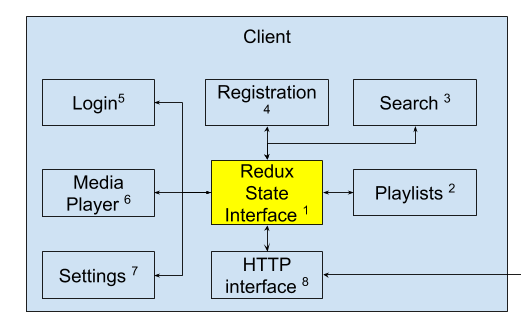
\includegraphics[width=0.60\textwidth]{images/client/client_redux.png}
 	\caption{Redux subsystem}
\end{figure}


\subsubsection{Subsystem Operating System}
We'll be using Chrome 42 or Firefox 39

\subsubsection{Subsystem Software Dependencies}
We will be using React-Redux v6.0.1 

\subsubsection{Subsystem Programming Languages}
We will be using JavaScript ES6

\subsubsection{Subsystem Data Structures}
We will have reducers and actions in Redux. The root reducer will contain the auth reducer, playlist reducer, and search reducer.

\subsubsection{Subsystem Data Processing}
We'll be using the fetch API to get data from the server in the form of JSON. It will return a JSON Ojbect back and compare it to the whole redux state and change the state where there are differences. 


\newpage
